\documentclass{article}
\usepackage{graphicx}
\usepackage{ amsmath , amssymb , amsthm }

% Finally the hyperref package is used for pdf files.
% This can be commented out for printed versions.
%\usepackage[pdfusetitle,colorlinks,plainpages=false]{hyperref} %colored links
\usepackage[pdfusetitle,hidelinks,plainpages=false]{hyperref} %noncolored links

%show only referenced equation numbers. use \eqref
\usepackage{mathtools}
\mathtoolsset{showonlyrefs=true}
%\usepackage[left]{showlabels}

%remove date
\date{}

%bibliography
\usepackage[sortcites,giveninits=true,backend=biber,style=ieee,style=numeric-comp]{biblatex}
\addbibresource{references.bib}

%no indent
\setlength{\parindent}{0pt}

\begin{document}

\title{Calculating the number of lines of text displayed on a monitor}

\maketitle

Call $n$ the number of lines of code (\textit{loc}) or of text displayed on a given monitor $M$. A monitor $M$ is specified by a tuple $M=(d,r_x,r_y,k)$, where $d > 0$ is the diagonal size, $r_x \in \mathbb{N}$ is the horizontal resolution (or number of pixels), $r_y \in \mathbb{N}$ is the vertical resolution, and $k \geq 1$ is the zoom level. Note that zoom levels less than $1$ are not allowed.

\section{Density}

In typography, the font size is measured in points (pt), where 1 pt = 1/72 inch. Computer displays work by lighting up pixels, so the font size needs to be expressed in pixels rather than in length. However, the physical size of a pixel varies among different monitors because of two factors:
\begin{itemize}
\item the resolution, that is, $r_x$ and $r_y$,
\item the screen physical size, expressed by its diagonal $d$.
\end{itemize}
To capture this idea, we define the \textit{density} $\delta$ of a monitor $M$ as
\begin{equation} \label{delta}
\delta = \frac{\sqrt{r_x^2+r_y^2}}{d}.
\end{equation}
The density is measured in pixels per inch (ppi).

In the Windows operating system, the font size expressed in pt and the number of vertical pixels $y$ required to draw a character are related by the formula \cite{win-dpi}:
\begin{equation} \label{y-fontsize}
y(\text{font size}) = \frac{\text{font size (pt)}}{72 \text{ inch}} * 120 \text{ ppi}
\end{equation}
Note that, in \cite{win-dpi}, it is written that Windows use 96 ppi, instead of 120 ppi, to perform the above conversion. However, experimentally it was noticed that 120 ppi is closer to the actual conversion that Windows 10 is performing. 

\section{Readability}

To ensure good readability, it is important to carefully choose the right character height for displayed text. Let $x$ be the height of a character. $x$ is expressed in inches. Among other factors, $x$ depends on the distance between the viewer and the display: the further the viewer is, the larger it should be. This relationship is expressed using the angle $A$ in the following figure:

\begin{figure}[!h]
   \centering
   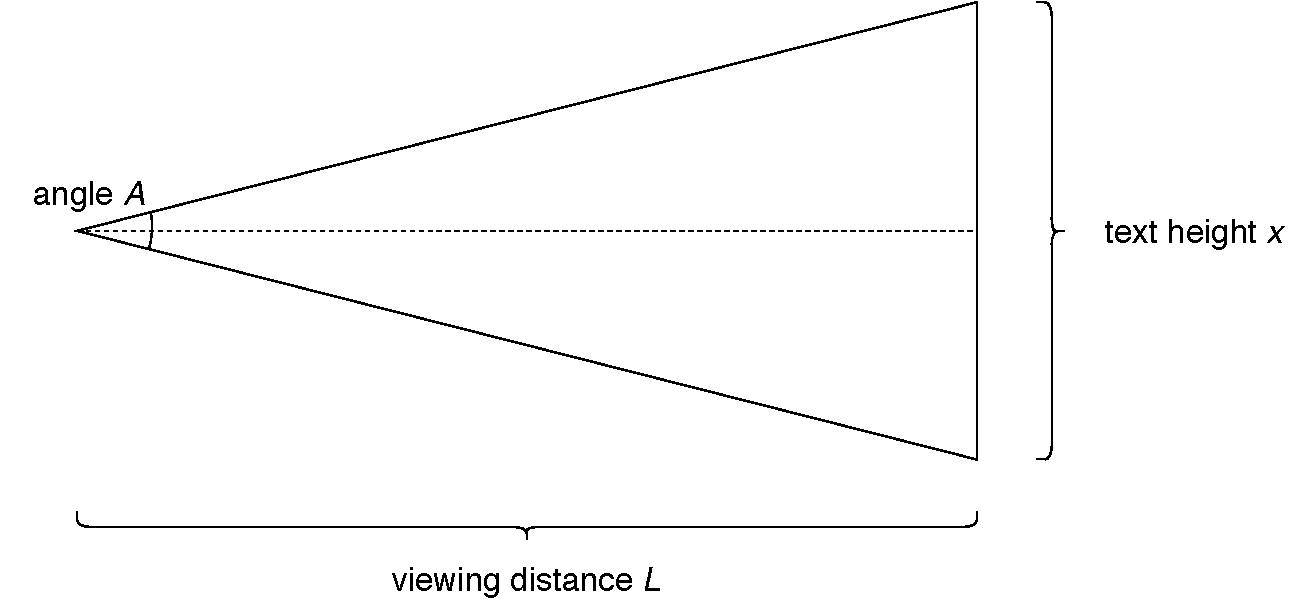
\includegraphics[page=1,width=0.8\textwidth]{angle.pdf}
 \caption{Relationship between the angle $A$, the viewing distance and the height of a character.}
 \label{fig:arch}
\end{figure}

The angle $A$ is usually expressed in arcminutes. 1 arcminute is 1/60 of 1 degree. $A$ can be then computed by the formula
\begin{equation}
A \text{ (arcminute)} = 60 * arctan \left( \frac{x}{L} \right).
\end{equation}
It is recommended to use at least 15 to 20 arcminutes \cite{extron}. For comparison, the angular acuity, which is the resolution of an eye, of a 10/10 eye is 1 arcminute \cite{wiki-va}.

\section{Computing the number of lines of text}
Turning to the number of lines of text of a monitor, each line uses a certain number $y$ of vertical pixels. The number of lines of text shown in a monitor $M$ is therefore:
\begin{equation} \label{n}
n = \frac{r_y}{y}.
\end{equation}

Given the height $x$ of a line, the number of vertical pixels required to draw that line is:
\begin{equation} \label{y}
y = x \delta.
\end{equation}

Expanding Equation \eqref{n} using Equations \eqref{delta} and \eqref{y}:
\begin{equation} \label{n-expanded}
n = \frac{r_y}{y} = \frac{r_y}{x\delta} = \frac{r_yd}{x\sqrt{r_x^2+r_y^2}}.
\end{equation}

The number of lines of text increases when the vertical resolution increases and it decreases when the line height increases. It also decreases when the density increases, having fixed the resolution and $x$. Indeed, increasing $\delta$ while keeping the resolution fixed means decreasing the diagonal of the monitor, which leads to a lower number of lines of text that can be displayed. In other words, $n$ increases when increasing the diagonal of the monitor. The increase has clearly a maximum, which is explained in Subsection \ref{details}. 

\section{Zoom level}
Windows 10 provides display scaling, which can increase the size of text and objects to make them easier to see on high PPI monitors. Windows uses a scale factor relative to a standard desktop of 96 PPI sitting at a 28 inch distance of the viewer \cite{build}. Here, the scale factor, also called the zoom level, is computed relative to the number $\bar{y}$ of vertical pixels used by a font size of 11 pt according to Equation \ref{y-fontsize}:
\begin{equation}
\bar{y} = y(11) = \frac{11}{72}*120 = \frac{55}{3} = 18.\bar{3} \text{ px}
\end{equation}
The above value will not be used directly in the following, so it is kept as a decimal value for convenience.

Given the number of pixels $y$ needed to draw one character, the zoom level is then:
\begin{equation} \label{k}
k = \frac{y}{\bar{y}}.
\end{equation}
Note that $y$ can be computed using Equation \eqref{y}. If $k$ is known, one can write Equation \eqref{n} as:
\begin{equation}
n = \frac{r_y}{k\bar{y}}.
\end{equation}

\subsection{Details} \label{details}
When writing software to compute $n$, some constraints must be considered. First of all, $k \geq 1$, so, from Equation \eqref{k}:
\begin{equation}
y \geq \bar{y}.
\end{equation}
Secondly, $y$ cannot exceed $r_y$. To take into account these constraint, Equation \eqref{y} is rewritten as:
\begin{equation}
y = 
\begin{cases}
    x\delta,  & \text{if } x\delta \geq \bar{y} \land x\delta \leq r_y \\
    \bar{y},  & \text{if } x\delta < \bar{y} \\
	r_y,      & \text{if } x\delta > r_y.
\end{cases}
\end{equation}

Therefore, Equation \eqref{n-expanded} is rewritten as:
\begin{equation}
n = 
\begin{cases}
    \frac{r_yd}{x\sqrt{r_x^2+r_y^2}},  & \text{if } x\delta \geq \bar{y} \land x\delta \leq r_y \\
    \frac{r_y}{\bar{y}},  & \text{if } x\delta < \bar{y} \\
	1,      & \text{if } x\delta > r_y.
\end{cases}
\end{equation}
In other words, $n$ cannot be smaller than 1 and cannot be larger than the number of lines of text whose height is equal to $\bar{y}$.

\printbibliography

\end{document}